\chapter{ANALISIS DAN PERANCANGAN SISTEM}
\section 


\tab Pada bab ini akan dijelaskan mengenai desain dan implementasi rancangan sistem informasi \textit{monitoring} SIK pada kegiatan relokasi ATM BRI. Sistem informasi \textit{Monitoring} SIK ini digunakan untuk \textit{memonitoring} jalannya kegiatan permintaan relokasi hingga selesai pengerjaan. Aplikasi ini dikhususkan untuk internal BRI dan provider penyedia jasa layanan dalam penanganan relokasi ATM BRI.

\section{Mengelola Request Relokasi}
Berikut adalah deskripsi sistem dan diagram aktivitas pada \textit{use case} Mengelola Request Relokasi. 
\subsection{Deskripsi Umum Sistem}
\tab Sistem akan melakukan pengelolaan request relokasi. Data yang dimasukkan akan disimpan ke dalam basis data. Pada kegiatan ini, terdapat sebuah parameter berupa kegiatan yang akan dilakukan pada saat relokasi ATM yaitu relokasi, instalasi dan reposisi.
\subsection{\textit{Use Case} dan Fitur Sistem}
Gambar \ref{figure:use_case_mengelola_req_relokasi} adalah \textit{use case} mengelola permintaan relokasi. Pada pengelolaan permintaan relokasi, user dapat melakukan beberapa kegiatan sebagai berikut:
	\subsubsection{Menambah Request Relokasi}
	User dapat menambahkan permintaan relokasi. Diagram \ref{figure:activity_menambah_req_relokasi} adalah diagram aktivitas menambah permintaan relokasi pada sistem \textit{Monitoring} SIK. Pada pengisian form permintaan relokasi ini, terdapat tiga buah kegiatan yaitu relokasi, instalasi dan reposisi. Pada kegiatan relokasi, user diharuskan memasukkan lokasi asal dan lokasi tujuan dari ATM yang akan di relokasi. Sedangkan pada kegiatan instalasi dan reposisi, hanya lokasi asal yang dapat di isi oleh user.
	\begin{figure}[h]
	\centerline {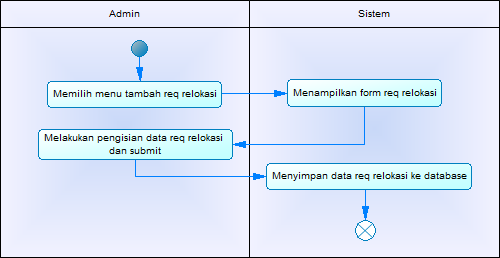
\includegraphics[width=9cm,height=6cm]{bab4/ActivityDiagram_MenambahkanReqRelokasi.png}}
	\caption{Diagram Aktivitas Menambah Request Relokasi}
	\label{figure:activity_menambah_req_relokasi}
	\end{figure}
		
	\subsubsection{Mengubah Request Relokasi}
	User dapat mengubah permintaan relokasi. Diagram \ref{figure:activity_mengubah_req_relokasi} adalah diagram aktivitas mengubah permintaan relokasi pada sistem \textit{Monitoring} SIK.
	\begin{figure}[h]
	\centerline {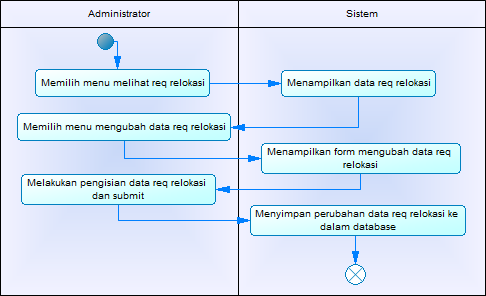
\includegraphics[width=9cm,height=5cm]{bab4/ActivityDiagram_MengubahReqRelokasi.png}}
	\caption{Diagram Aktivitas Mengubah Request Relokasi}
	\label{figure:activity_mengubah_req_relokasi}
	\end{figure}

	\subsubsection{Menghapus Request Relokasi}
	User dapat menghapus permintaan relokasi. Diagram \ref{figure:activity_menghapus_req_relokasi} adalah diagram aktivitas menghapus permintaan relokasi pada sistem \textit{Monitoring} SIK.
	\begin{figure}[h]
	\centerline {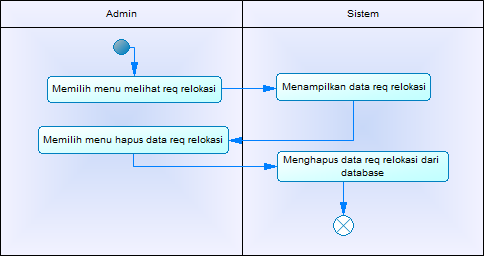
\includegraphics[width=9cm,height=5cm]{bab4/ActivityDiagram_MenghapusReqRelokasi.png}}
	\caption{Diagram Aktivitas Menghapus Request Relokasi}
	\label{figure:activity_menghapus_req_relokasi}
	\end{figure}		

	\begin{figure}[h]
	\centerline {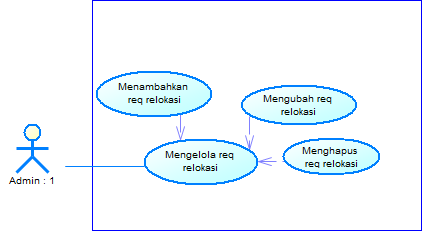
\includegraphics[width=8cm,height=4.5cm]{bab4/use-case-mengelola-req-relokasi.png}}
	\caption{Diagram \textit{Use Case} Mengelola Request Relokasi}
	\label{figure:use_case_mengelola_req_relokasi}
	\end{figure}

\section{Mengelola SIK}
Berikut adalah deskripsi dan diagram aktivitas pada \textit{use case} Mengelola SIK.
\subsection{Deskripsi Umum Sistem}
\tab Sistem ini akan melakukan pengelolaan SIK(Surat Izin Kerja). Pembuatan SIK didasarkan pada permintaan relokasi yang ada pada daftar permintaan relokasi. Daftar-daftar permintaan relokasi yang telah dibuatkan SIK tidak akan dimunculkan kembali pada saat pengisian formulir penambahan SIK. Data yang dimasukkan akan disimpan ke dalam basis data.
\subsection{\textit{Use Case} dan Fitur Sistem}
Gambar \ref{figure:use_case_mengelola_sik} adalah \textit{use case} mengelola SIK. Pada pengelolaan SIK, user dapat melakukan beberapa kegiatan sebagai berikut:
	\subsubsection{Menambah SIK}
	User dapat menambahkan SIK berdasarkan permintaan relokasi yang ada. Batasan dalam pembuatan SIK yaitu setiap SIK harus dikerjakan oleh provider yang sama. Pada saat pembuatan SIK, permintaan relokasi yang telah dibuatkan SIK tidak akan ditampilkan ulang pada daftar permintaan relokasi yang ada. Diagram \ref{figure:activity_menambah_sik} adalah diagram aktivitas menambah SIK pada sistem \textit{Monitoring} SIK.
	\begin{figure}[h]
	\centerline {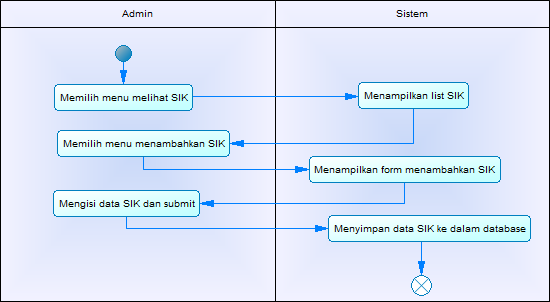
\includegraphics[width=9cm,height=6cm]{bab4/ActivityDiagram_MenambahkanSIK.png}}
	\caption{Diagram Aktivitas Menambah SIK}
	\label{figure:activity_menambah_sik}
	\end{figure}
		
	\subsubsection{Mengubah SIK}
	User dapat mengubah data SIK yang telah ditambahkan. Diagram \ref{figure:activity_mengubah_sik} adalah diagram aktivitas mengubah SIK pada sistem Monitoring SIK.
	\begin{figure}[h]
	\centerline {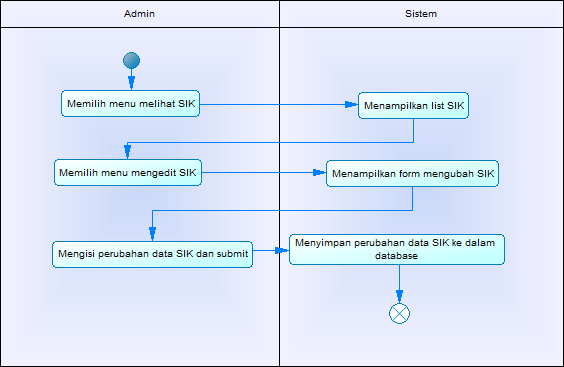
\includegraphics[width=9cm,height=5.6cm]{bab4/ActivityDiagram_MengubahSIK.png}}
	\caption{Diagram Aktivitas Mengubah SIK}
	\label{figure:activity_mengubah_sik}
	\end{figure}

	\subsubsection{Menghapus SIK}
	User dapat menghapus SIK. Pada penghapusan SIK, permintaan relokasi yang SIKnya dihapus akan ditampilkan ulang pada daftar permintaan relokasi. Diagram \ref{figure:activity_menghapus_sik} adalah diagram aktivitas menghapus SIK pada sistem \textit{Monitoring } SIK.
	\begin{figure}[h]
	\centerline {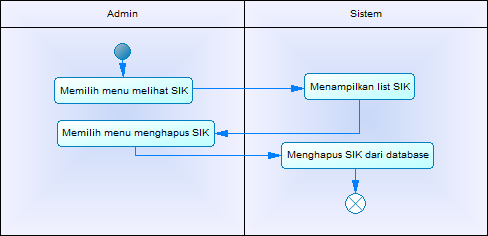
\includegraphics[width=9cm,height=4.5cm]{bab4/ActivityDiagram_MenghapusSIK.png}}
	\caption{Diagram Aktivitas Menghapus SIK}
	\label{figure:activity_menghapus_sik}
	\end{figure}		

	\begin{figure}[h]
	\centerline {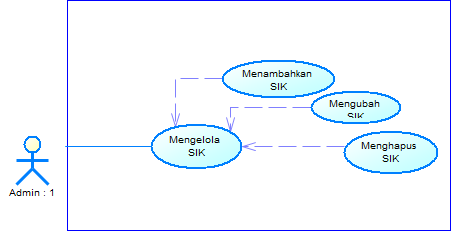
\includegraphics[width=9cm,height=5cm]{bab4/use-case-mengelola-sik.png}}
	\caption{Diagram \textit{Use Case} Mengelola SIK}
	\label{figure:use_case_mengelola_sik}
	\end{figure}

\section{Mengelola Eksekusi}
Berikut adalah deskripsi dan diagram aktivitas pada \textit{use case} Mengelola Eksekusi.
\subsection{Deskripsi Umum Sistem}
\tab Sistem ini akan melakukan pengelolaan eksekusi permintaan relokasi. Pengelolaan eksekusi permintaan relokasi didasarkan pada SIK yang telah dibuat. Apabila SIK sudah masuk tahap \textit{approval} oleh kepala divisi, selanjutkan masuk pada tahap eksekusi.
\subsection{\textit{Use Case} dan Fitur Sistem}
Gambar \ref{figure:use_case_mengelola_eksekusi} adalah \textit{use case} mengelola eksekusi permintaan relokasi. Pada pengelolaan eksekusi permintaan relokasi, user dapat melakukan beberapa kegiatan sebagai berikut:
	\subsubsection{Menambah Eksekusi}
	User dapat menambahkan eksekusi permintaan relokasi berdasarkan pada SIK yang ada. Penambahan eksekusi dilakukan dengan pengubahan status SIK dari proses menjadi \textit{approved}. Diagram \ref{figure:activity_menambah_eksekusi} adalah diagram aktivitas menambah eksekusi request relokasi pada sistem \textit{Monitoring} SIK.
	\begin{figure}[h]
	\centerline {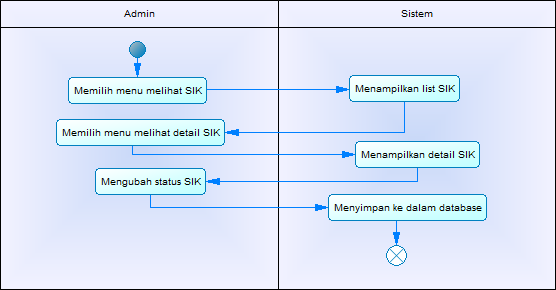
\includegraphics[width=9cm,height=6cm]{bab4/ActivityDiagram_MenambahkanEksekusi.png}}
	\caption{Diagram Aktivitas Menambah Eksekusi Request Relokasi}
	\label{figure:activity_menambah_eksekusi}
	\end{figure}
		
	\subsubsection{Mengubah Eksekusi}
	User dapat mengubah eksekusi permintaan relokasi yang telah dibuat. Perubahan pada data eksekusi akan disimpan menggantikan data yang sebelumnya telah dibuat. Diagram \ref{figure:activity_mengubah_eksekusi} adalah diagram aktivitas mengubah eksekusi permintaan relokasi pada sistem \textit{Monitoring} SIK.
	\begin{figure}[h]
	\centerline {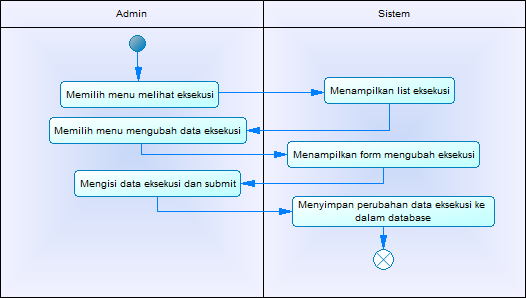
\includegraphics[width=9cm,height=4.6cm]{bab4/ActivityDiagram_MengubahEksekusi.png}}
	\caption{Diagram Aktivitas Mengubah Eksekusi Request Relokasi}
	\label{figure:activity_mengubah_eksekusi}
	\end{figure}

	\subsubsection{Menghapus Eksekusi}
	User dapat menghapus eksekusi permintaan relokasi. Dan mengembalikan status eksekusi menjadi proses pembuatan SIK. Diagram \ref{figure:activity_menghapus_eksekusi} adalah diagram aktivitas menghapus eksekusi permintaan relokasi pada sistem \textit{Monitoring} SIK.
	\begin{figure}[h]
	\centerline {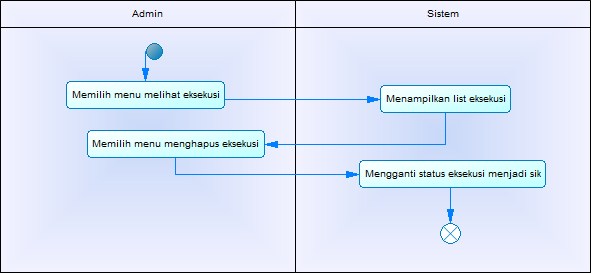
\includegraphics[width=9cm,height=4.5cm]{bab4/ActivityDiagram_MenghapusEksekusi.png}}
	\caption{Diagram Aktivitas Menghapus Eksekusi Request Relokasi}
	\label{figure:activity_menghapus_eksekusi}
	\end{figure}		

	\begin{figure}[h]
	\centerline {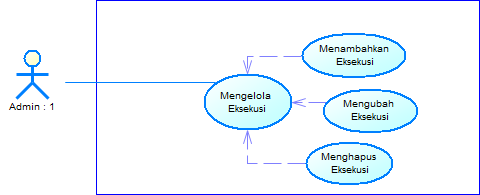
\includegraphics[width=9cm,height=5cm]{bab4/use-case-mengelola-eksekusi.png}}
	\caption{Diagram \textit{Use Case} Mengelola Eksekusi Request Relokasi}
	\label{figure:use_case_mengelola_eksekusi}
	\end{figure}

\section{Mengelola Penagihan}
Berikut adalah deskripsi dan diagram aktivitas pada \textit{use case} Mengelola Penagihan.
\subsection{Deskripsi Umum Sistem}
\tab Sistem ini akan melakukan pengelolaan penagihan permintaan relokasi. Pengelolaan penagihan permintaan relokasi didasarkan pada proses sebelumnya. Setelah proses eksekusi selesai, status SIK akan diubah menjadi penagihan pembayaran.
\subsection{\textit{Use Case} dan Fitur Sistem}
Gambar \ref{figure:use_case_mengelola_penagihan} adalah \textit{use case} mengelola penagihan permintaan relokasi. Pada pengelolaan penagihan permintaan relokasi, user dapat melakukan beberapa kegiatan sebagai berikut:
	\subsubsection{Menambah Penagihan}
	User dapat menambahkan penagihan permintaan relokasi. Berdasarkan pada proses sebelumnya, yaitu eksekusi. Penambahan proses penagihan dilakukan dengan pengubahan status SIK dari eksekusi menjadi penagihan. Diagram \ref{figure:activity_menambah_penagihan} adalah diagram aktivitas menambah penagihan permintaan relokasi pada sistem \textit{Monitoring} SIK.
	\begin{figure}[h]
	\centerline {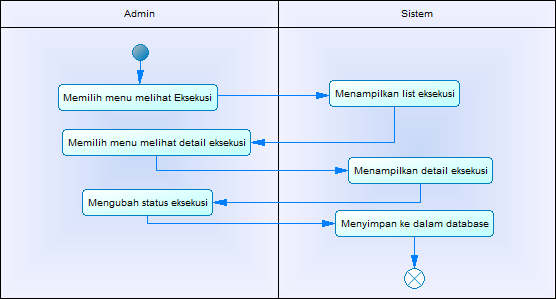
\includegraphics[width=9cm,height=4.6cm]{bab4/ActivityDiagram_MenambahkanPenagihan.png}}
	\caption{Diagram Aktivitas Menambah Penagihan Request Relokasi}
	\label{figure:activity_menambah_penagihan}
	\end{figure}
	\subsubsection{Mengubah Penagihan}
	User dapat mengubah penagihan permintaan relokasi yang telah dibuat. Perubahan penagihan yang dibuat akan menggantikan data yang sebelumnya dibuat. Diagram \ref{figure:activity_mengubah_penagihan} adalah diagram aktivitas mengubah penagihan permintaan relokasi pada sistem Monitoring SIK.
	\begin{figure}[h]
	\centerline {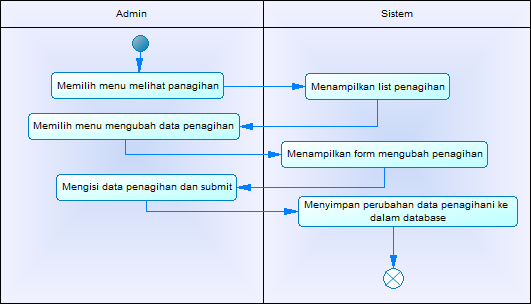
\includegraphics[width=9cm,height=6cm]{bab4/ActivityDiagram_MengubahPenagihan.png}}
	\caption{Diagram Aktivitas Mengubah Penagihan Request Relokasi}
	\label{figure:activity_mengubah_penagihan}
	\end{figure}
	
	\subsubsection{Menghapus Penagihan}
	User dapat menghapus penagihan permintaan relokasi. proses penghapusan data penagihan akan mengembalikan proses penagihan menjadi proses eksekusi. Diagram \ref{figure:activity_menghapus_penagihan} adalah diagram aktivitas menghapus penagihan permintaan relokasi pada sistem \textit{Monitoring} SIK.
	\begin{figure}[h]
	\centerline {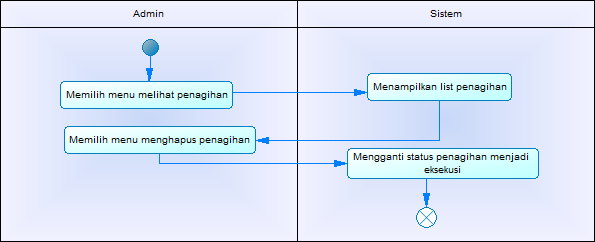
\includegraphics[width=9cm,height=4cm]{bab4/ActivityDiagram_MenghapusPenagihan.png}}
	\caption{Diagram Aktivitas Menghapus Penagihan Request Relokasi}
	\label{figure:activity_menghapus_penagihan}
	\end{figure}		

	\begin{figure}[h]
	\centerline {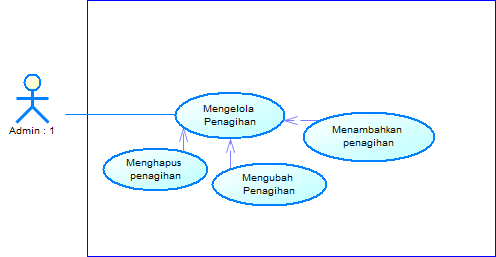
\includegraphics[width=9cm,height=5cm]{bab4/use-case-mengelola-penagihan.png}}
	\caption{Diagram \textit{Use Case} Mengelola Penagihan Request Relokasi}
	\label{figure:use_case_mengelola_penagihan}
	\end{figure}

\section{Melihat Request Relokasi}
Berikut adalah deskripsi dan diagram aktivitas pada \textit{use case} Melihat Request Relokasi.
\subsection{Deskripsi Umum Sistem}
\tab Sistem dapat menampilkan daftar permintaan relokasi kepada user berdasarkan \textit{record} yang tersimpan dalam basis data.
\subsection{\textit{Use Case} dan Fitur Sistem}
Gambar \ref{figure:use_case_melihat_req_relokasi} adalah \textit{use case} melihat daftar permintaan relokasi. Pada halaman melihat permintaan relokasi, user dapat melakukan beberapa kegiatan sebagai berikut:
	\subsubsection{Melihat Request Relokasi}
	User dapat melihat daftar permintaan relokasi yang telah ditambahkan ke dalam basis data. Diagram \ref{figure:activity_melihat_req_relokasi} adalah diagram aktivitas melihat daftar permintaan relokasi pada sistem \textit{Monitoring} SIK.
	\begin{figure}[h]
	\centerline {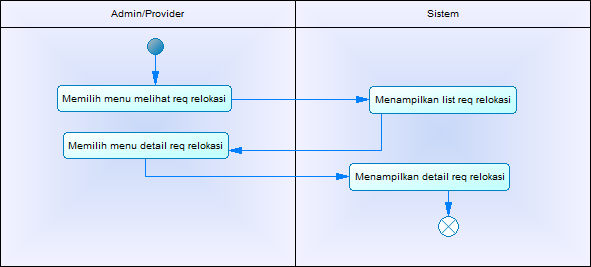
\includegraphics[width=9cm,height=4.5cm]{bab4/ActivityDiagram_MelihatReqRelokasi.png}}
	\caption{Diagram Aktivitas Melihat Daftar Request Relokasi}
	\label{figure:activity_melihat_req_relokasi}
	\end{figure}
	
	\subsubsection{Men\textit{download} Request Relokasi}
	User dapat men\textit{download} surat permintaan relokasi yang telah di\textit{upload} ke dalam basis data. Diagram \ref{figure:activity_mendownload_req_relokasi} adalah aktivitas diagram men\textit{download} surat permintaan relokasi pada sistem \textit{Monitoring} SIK.
	\begin{figure}[h]
	\centerline
	{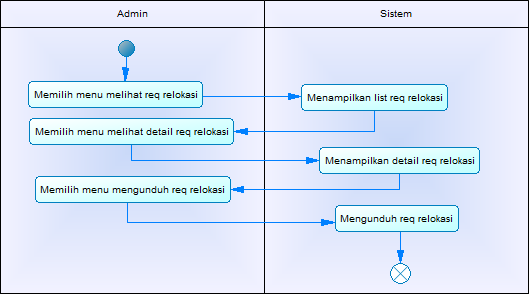
\includegraphics[width=9cm,height=5cm]{bab4/ActivityDiagram_DownloadReqRelokasi.png}}
	\caption{Diagram Aktivitas Mendownload Request Relokasi}
	\label{figure:activity_mendownload_req_relokasi}
	\end{figure}

	\begin{figure}[h]
	\centerline
	{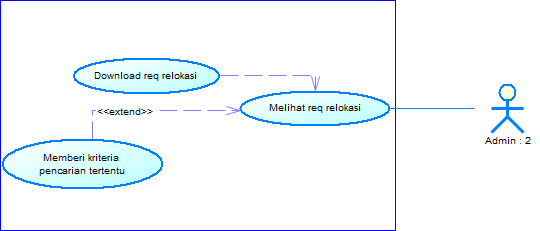
\includegraphics[width=9cm,height=5cm]{bab4/use-case-melihat-req-relokasi.png}}
	\caption{Diagram \textit{Use Case} Melihat Request Relokasi}
	\label{figure:use_case_melihat_req_relokasi}
	\end{figure}

\section{Melihat SIK}
Berikut adalah deskripsi dan diagram aktivitas pada \textit{use case} Melihat SIK.
\subsection{Deskripsi Umum Sistem}
\tab Sistem dapat menampilkan daftar SIK kepada user berdasarkan \textit{record} yang tersimpan dalam basis data.
\subsection{\textit{Use Case} dan Fitur Sistem}
Gambar \ref{figure:use_case_melihat_sik} adalah \textit{use case} melihat daftar SIK. Pada halaman melihat daftar SIK, user dapat melakukan beberapa kegiatan sebagai berikut:
	\subsubsection{Melihat SIK}
	User dapat melihat daftar SIK yang telah ditambahkan ke dalam basis data. Diagram \ref{figure:activity_melihat_sik} adalah diagram aktivitas melihat daftar SIK pada sistem \textit{Monitoring} SIK.
	\begin{figure}[h]
	\centerline {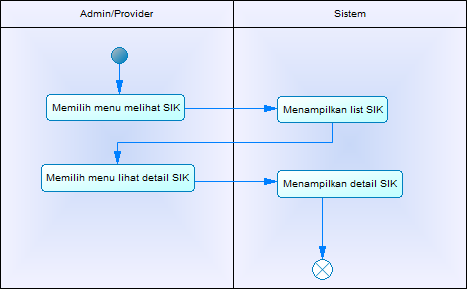
\includegraphics[width=9cm,height=5cm]{bab4/ActivityDiagram_MelihatSIK.png}}
	\caption{Diagram Aktivitas Melihat Daftar SIK}
	\label{figure:activity_melihat_sik}
	\end{figure}
	
	\subsubsection{Men\textit{download} SIK}
	User dapat men\textit{download} SIK yang telah di\textit{upload} ke dalam basis data. Diagram \ref{figure:activity_mendownload_sik} adalah aktivitas diagram men\textit{download} SIK pada sistem \textit{Monitoring} SIK.
	\begin{figure}[h]
	\centerline
	{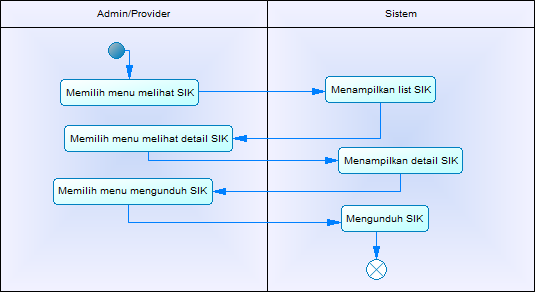
\includegraphics[width=9cm,height=5cm]{bab4/ActivityDiagram_DownloadSIK.png}}
	\caption{Diagram Aktivitas Mendownload SIK}
	\label{figure:activity_mendownload_sik}
	\end{figure}

	\begin{figure}[h]
	\centerline
	{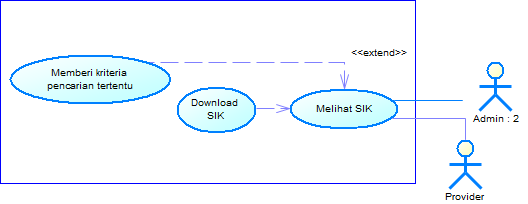
\includegraphics[width=9cm,height=5cm]{bab4/use-case-melihat-sik.png}}
	\caption{Diagram \textit{Use Case} Melihat SIK}
	\label{figure:use_case_melihat_sik}
	\end{figure}
	
\section{Melihat Eksekusi}
Berikut adalah deskripsi dan diagram aktivitas pada \textit{use case} Melihat Eksekusi.
\subsection{Deskripsi Umum Sistem}
\tab Sistem dapat menampilkan daftar eksekusi permintaan relokasi. Daftar eksekusi permintaan relokasi ditampilkan berdasarkan SIK yang memiliki status \textit{approval}.
\subsection{\textit{Use Case} dan Fitur Sistem}
Gambar \ref{figure:use_case_melihat_eksekusi} adalah \textit{use case} melihat daftar eksekusi permintaan relokasi. Pada halaman melihat daftar eksekusi permintaan relokasi, user dapat melakukan beberapa kegiatan sebagai berikut:
	\subsubsection{Melihat Ekekusi}
	User dapat melihat daftar eksekusi permintaan relokasi berdasarkan daftar SIK dengan status \textit{approval}. Diagram \ref{figure:activity_melihat_eksekusi} adalah diagram aktivitas melihat daftar eksekusi permintaan relokasi pada sistem \textit{Monitoring} SIK.
	\begin{figure}[h]
	\centerline {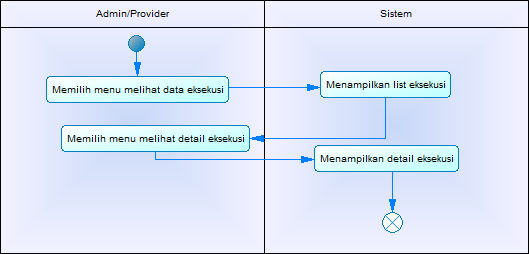
\includegraphics[width=9cm,height=4.6cm]{bab4/ActivityDiagram_MelihatEksekusi.png}}
	\caption{Diagram Aktivitas Melihat Daftar Eksekusi}
	\label{figure:activity_melihat_eksekusi}
	\end{figure}
	
	\subsubsection{Men\textit{download} Berita Acara}
	User dapat men\textit{download} berita acara yang telah di\textit{upload} ke dalam basis data. Diagram \ref{figure:activity_mendownload_berita_acara} adalah aktivitas diagram men\textit{download} berita acara pada sistem \textit{Monitoring} SIK.
	\begin{figure}[h]
	\centerline
	{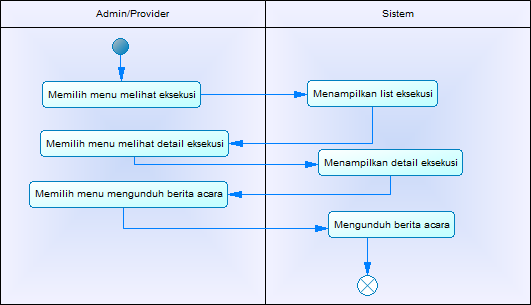
\includegraphics[width=9cm,height=4.6cm]{bab4/ActivityDiagram_DownloadBeritaAcara.png}}
	\caption{Diagram Aktivitas Mendownload Berita Acara}
	\label{figure:activity_mendownload_berita_acara}
	\end{figure}
	
	\subsubsection{Men\textit{download} Tagihan}
	User dapat men\textit{download} penagihan pembayaran yang telah di\textit{upload} ke dalam basis data. Diagram \ref{figure:activity_mendownload_tagihan} adalah aktivitas diagram men\textit{download} penagihan pembayaran pada sistem \textit{Monitoring} SIK.
	\begin{figure}[h]
	\centerline
	{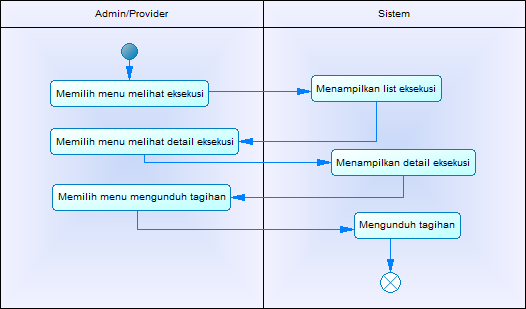
\includegraphics[width=9cm,height=5cm]{bab4/ActivityDiagram_DownloadTagihan.png}}
	\caption{Diagram Aktivitas Mendownload Tagihan Pembayaran}
	\label{figure:activity_mendownload_tagihan}
	\end{figure}

	\begin{figure}[h!]
	\centerline
	{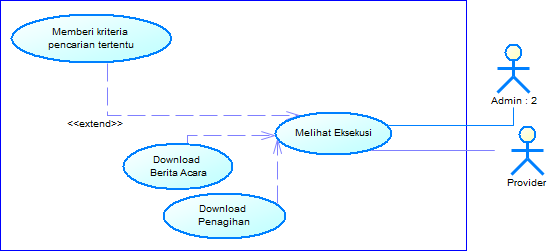
\includegraphics[width=9cm,height=5cm]{bab4/use-case-melihat-eksekusi.png}}
	\caption{Diagram \textit{Use Case} Melihat Eksekusi}
	\label{figure:use_case_melihat_eksekusi}
	\end{figure}
	
\section{Melihat Penagihan}
Berikut adalah deskripsi dan diagram aktivitas pada \textit{use case} Melihat Penagihan.
\subsection{Deskripsi Umum Sistem}
\tab Sistem dapat menampilkan daftar penagihan pembayaran permintaan relokasi. Daftar penagihan pembayaran permintaan relokasi didasarkan pada proses eksekusi yang memiliki status \textit{finish}. Pada halaman ini, user dapat melihat proses-proses penagihan pembayaran dari kegiatan-kegiatan relokasi yang dikerjakan.
\subsection{\textit{Use Case} dan Fitur Sistem}
Gambar \ref{figure:use_case_melihat_penagihan} adalah \textit{use case} melihat daftar penagihan pembayaran permintaan relokasi. Pada halaman melihat daftar penagihan pembayaran permintaan relokasi, user dapat melakukan beberapa kegiatan sebagai berikut:
	\subsubsection{Melihat Penagihan}
	User dapat melihat daftar penagihan pembayaran permintaan relokasi berdasarkan daftar proses eksekusi dengan status \textit{finish}. Diagram \ref{figure:activity_melihat_penagihan} adalah diagram aktivitas melihat daftar penagihan pembayaran permintaan relokasi pada sistem \textit{Monitoring} SIK.
	
	\begin{figure}[h!]
	\centerline {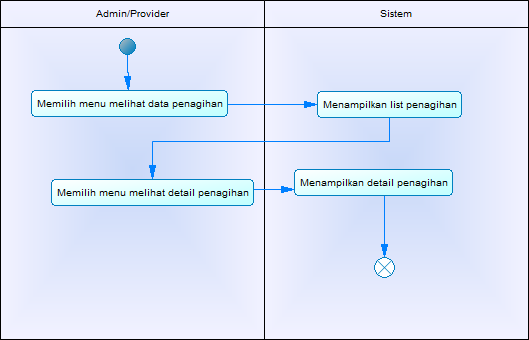
\includegraphics[width=9cm,height=5cm]{bab4/ActivityDiagram_MelihatPenagihan.png}}
	\caption{Diagram Aktivitas Melihat Daftar Penagihan Pembayaran}
	\label{figure:activity_melihat_penagihan}
	\end{figure}

	\begin{figure}[h!]
	\centerline
	{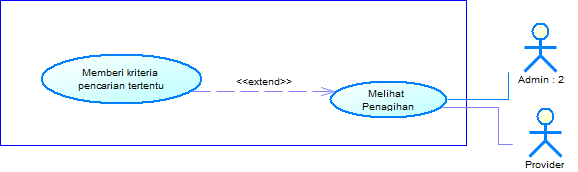
\includegraphics[width=9cm,height=5.5cm]{bab4/use-case-melihat-penagihan.png}}
	\caption{Diagram \textit{Use Case} Melihat Penagihan Pembayaran}
	\label{figure:use_case_melihat_penagihan}
	\end{figure}
	
\section{Melihat Finish}
Berikut adalah deskripsi dan diagram aktivitas pada \textit{use case} Melihat Finish.
\subsection{Deskripsi Umum Sistem}
\tab Sistem dapat menampilkan daftar permintaan relokasi dengan status telah dibayar.
\subsection{\textit{Use Case} dan Fitur Sistem}
Gambar \ref{figure:use_case_melihat_finish} adalah \textit{use case} melihat daftar permintaan relokasi dengan status telah dibayar. Pada halaman melihat daftar permintaan relokasi dengan status telah dibayar, user dapat melakukan beberapa kegiatan sebagai berikut:
	\subsubsection{Melihat Finish}
	User dapat melihat daftar permintaan relokasi dengan status telah dibayar. Diagram \ref{figure:activity_melihat_finish} adalah diagram aktivitas melihat daftar penagihan pembayaran permintaan relokasi pada sistem \textit{Monitoring} SIK.
	\begin{figure}[h]
	\centerline {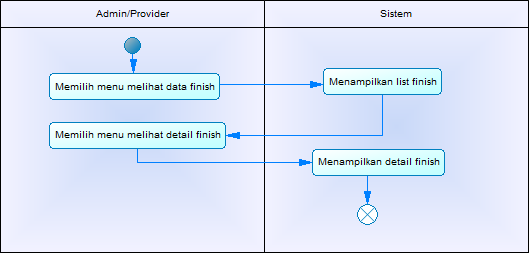
\includegraphics[width=9cm,height=5.5cm]{bab4/ActivityDiagram_MelihatFinish.png}}
	\caption{Diagram Aktivitas Melihat Daftar Permintaan Relokasi Sudah Dibayar}
	\label{figure:activity_melihat_finish}
	\end{figure}

	\begin{figure}[h!]
	\centerline
	{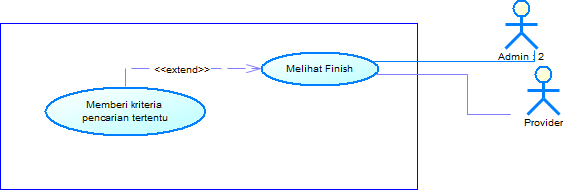
\includegraphics[width=9cm,height=5cm]{bab4/use-case-melihat-finish.png}}
	\caption{Diagram \textit{Use Case} Melihat Daftar Permintaan Relokasi Sudah Dibayar}
	\label{figure:use_case_melihat_finish}
	\end{figure}
	
\newpage
\section{Perancangan Data}
\tab Dalam pembuatan sebuah sistem informasi, database merupakan salah satu faktor utama yang penting. Perancangan dan alur data pada sebuah sistem harus dapat memenuhi kebutuhan-kebutuhan sistem, meliputi penambahan data, perubahan isi data dan penghapusan data dari basisdata sistem. Berikut adalah perancangan data pada sistem informasi \textit{monitoring} SIK.
\subsection{\textit{Conceptual Data Model}}
CDM (\textit{Conceptual Data Model}) merupakan sebuah model yang didasarkan pada objek-objek di dunia nyata. Objek dasar tersebut direpresentasikan dalam bentuk \textit{entity relationship diagram}. Gambar \ref{figure:CDM} adalah CDM pada pembuatan sistem informasi \textit{monitoring} SIK.
	\begin{figure}[h!]
	\centerline
	{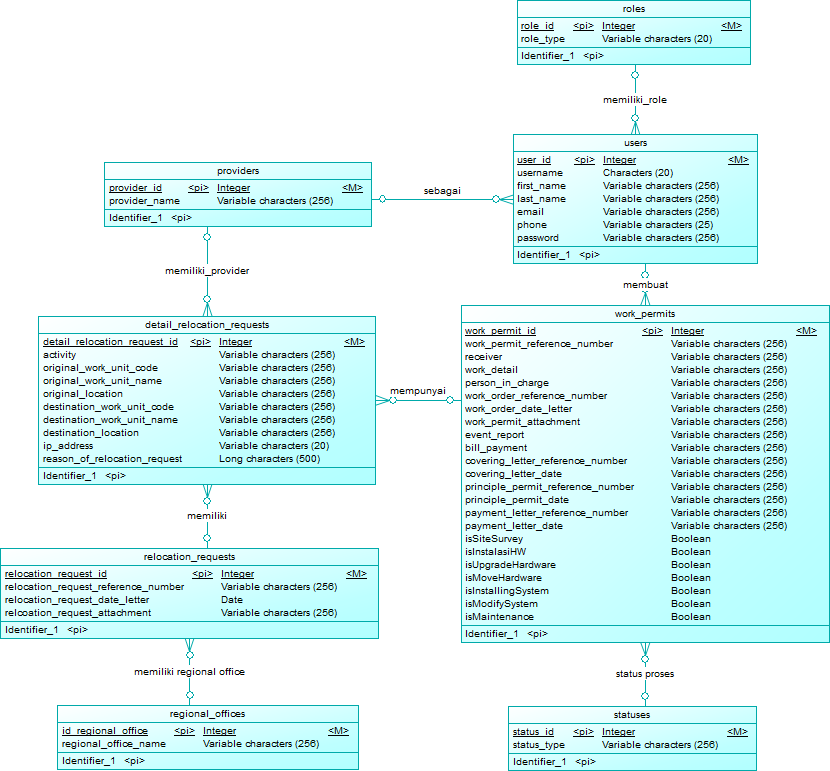
\includegraphics[width=10cm,height=14cm]{bab4/CDM.png}}
	\caption{Diagram \textit{Conceptual Data Model}}
	\label{figure:CDM}
	\end{figure}
	
\subsection{\textit{Physical Data Model}}
PDM (\textit{Physical Data Model}) adalah model yang digambarkan dalam sebuah tabel serta hubungan-hubungan antara data dengan tabel lain. Gambar \ref{figure:PDM} adalah PDM pada pembuatan sistem informasi \textit{monitoring} SIK.
	\begin{figure}[h!]
	\centerline
	{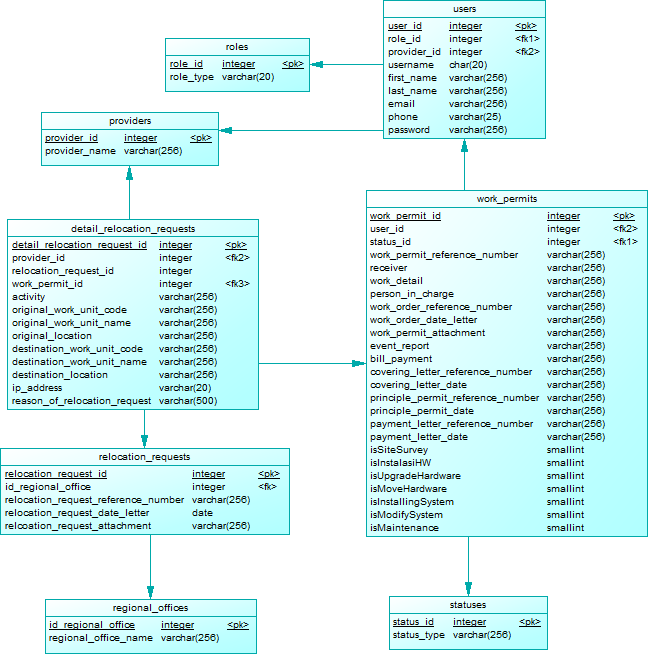
\includegraphics[width=10cm,height=11cm]{bab4/PDM.png}}
	\caption{Diagram \textit{Physical Data Model}}
	\label{figure:PDM}
	\end{figure}